\documentclass[a4paper,12pt]{article}

%%% Работа с русским языком
\usepackage{cmap}					% поиск в PDF
\usepackage{mathtext} 				% русские буквы в формулах
\usepackage[T2A]{fontenc}			% кодировка
\usepackage[utf8]{inputenc}			% кодировка исходного текста
\usepackage[english,russian]{babel}	% локализация и переносы
\usepackage{xcolor}
\usepackage{hyperref}
 % Цвета для гиперссылок
\definecolor{linkcolor}{HTML}{799B03} % цвет ссылок
\definecolor{urlcolor}{HTML}{799B03} % цвет гиперссылок

\hypersetup{pdfstartview=FitH,  linkcolor=linkcolor,urlcolor=urlcolor, colorlinks=true}

%%% Дополнительная работа с математикой
\usepackage{amsfonts,amssymb,amsthm,mathtools} % AMS
\usepackage{amsmath}
\usepackage{icomma} % "Умная" запятая: $0,2$ --- число, $0, 2$ --- перечисление

%% Номера формул
%\mathtoolsset{showonlyrefs=true} % Показывать номера только у тех формул, на которые есть \eqref{} в тексте.

%% Шрифты
\usepackage{euscript}	 % Шрифт Евклид
\usepackage{mathrsfs} % Красивый матшрифт

%% Свои команды
\DeclareMathOperator{\sgn}{\mathop{sgn}}

%% Перенос знаков в формулах (по Львовскому)
\newcommand*{\hm}[1]{#1\nobreak\discretionary{}
{\hbox{$\mathsurround=0pt #1$}}{}}
% графика
\usepackage{graphicx}

\usepackage[left=25mm, top=30mm, right=25mm, bottom=30mm, nohead, nofoot]{geometry}

\graphicspath{{pictures/}}
\DeclareGraphicsExtensions{.pdf,.png,.jpg}
\author{Бурмашев Григорий, БПМИ-208}
\title{Язык SQP, домашнее задание 10}
\date{\today}
\begin{document}
\maketitle
\clearpage
\section*{Номер 12} 
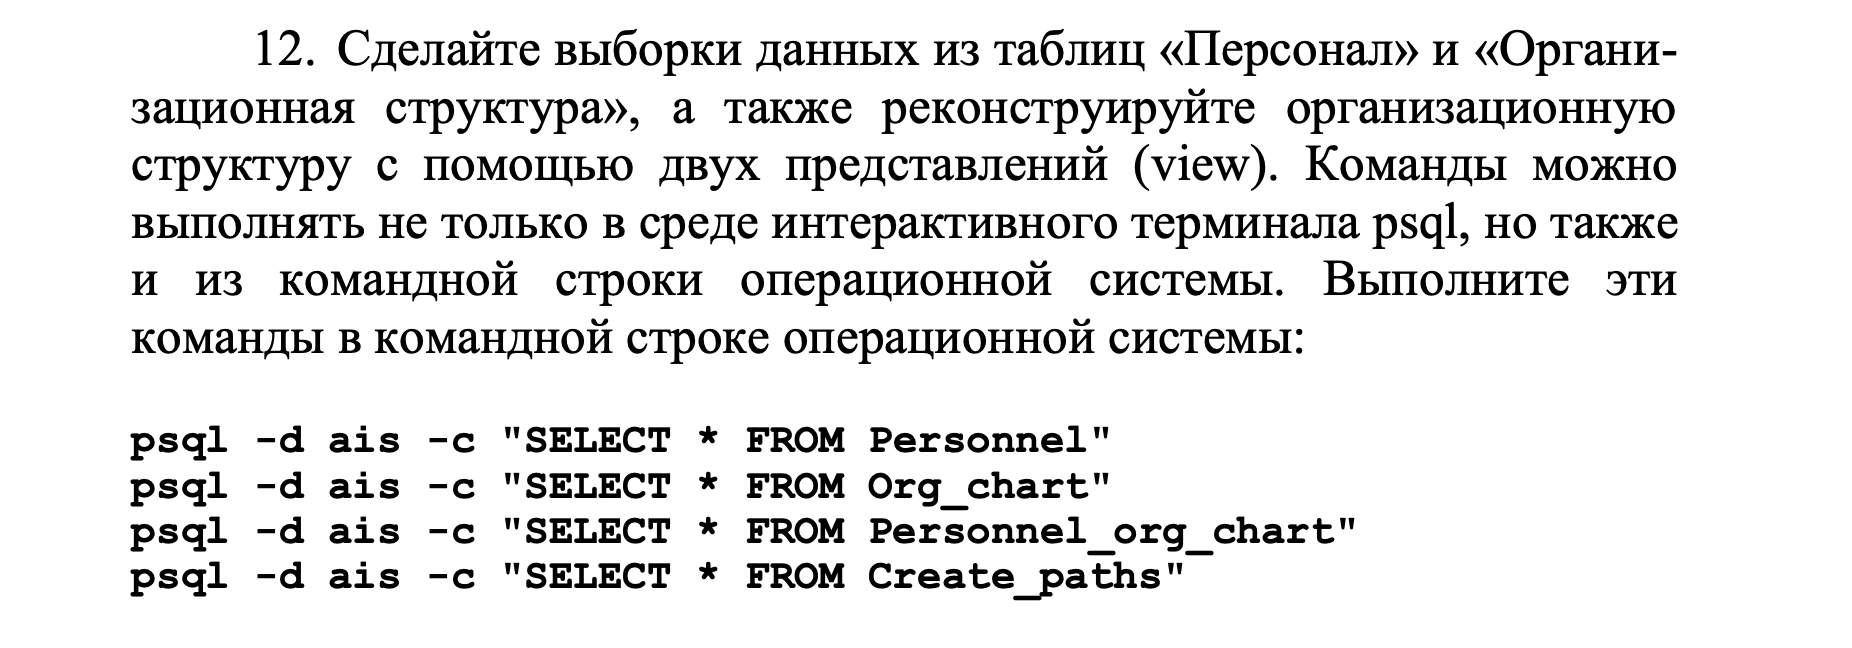
\includegraphics[scale=0.5]{12_1.png}
\clearpage
\begin{center}
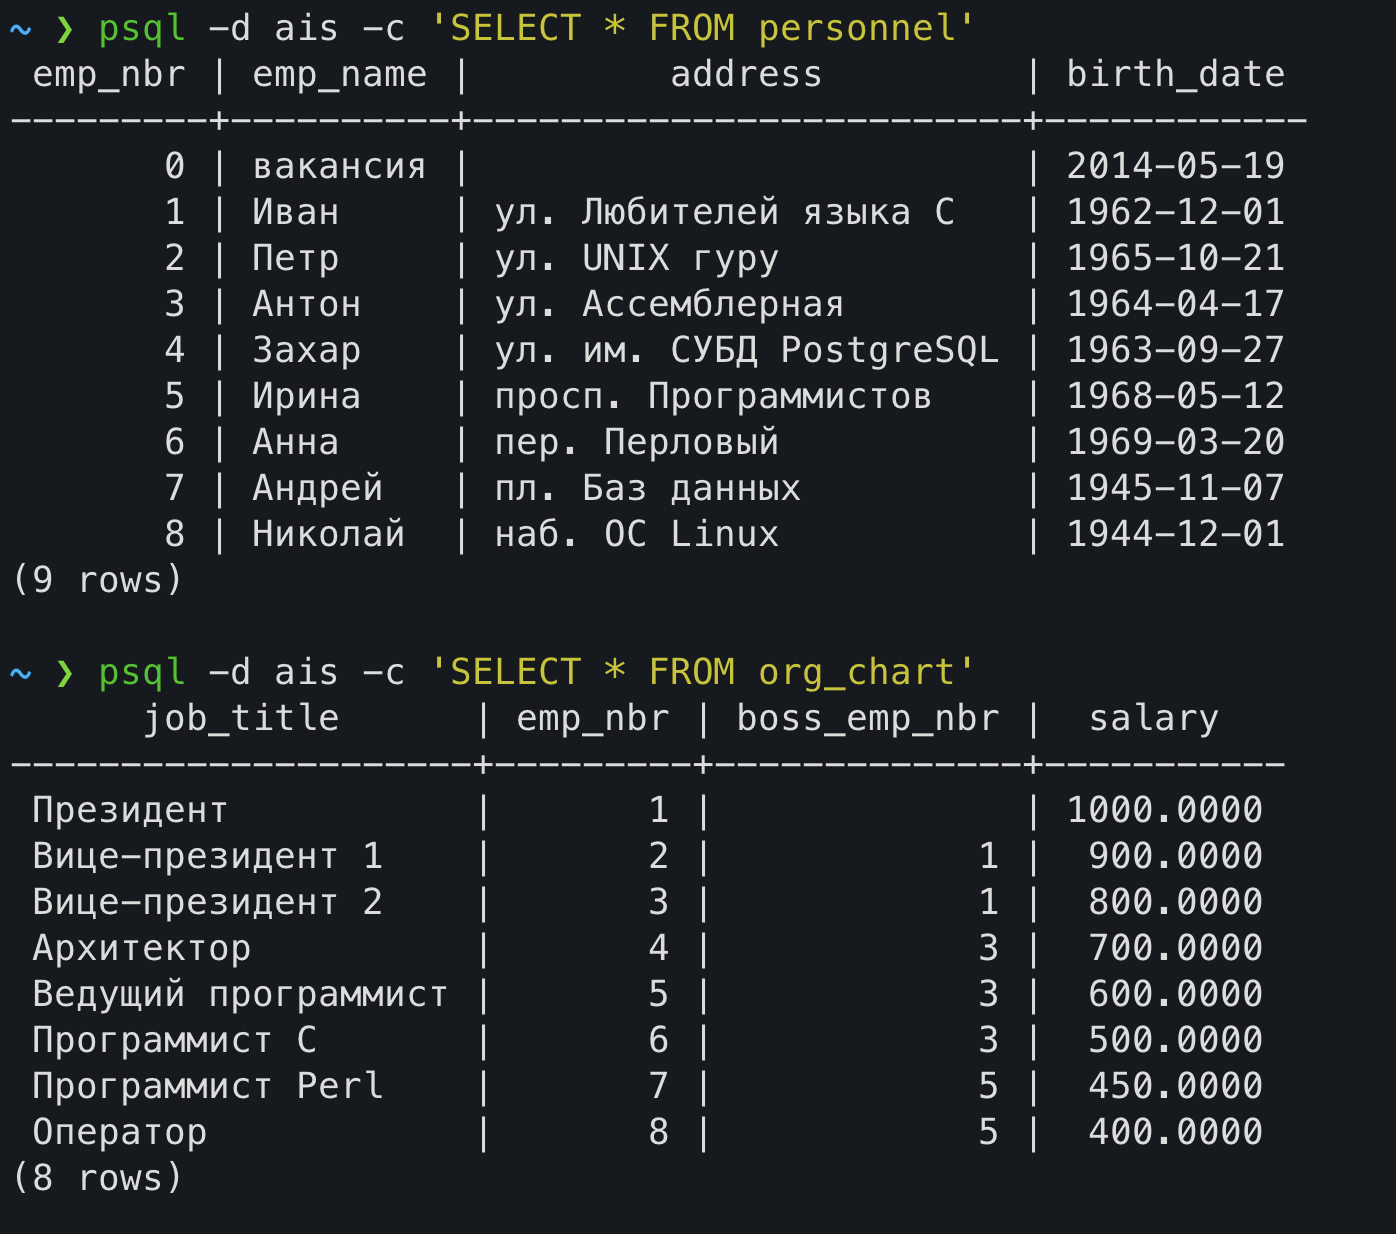
\includegraphics[scale=0.7]{12_2.png}
\end{center}
\begin{center}
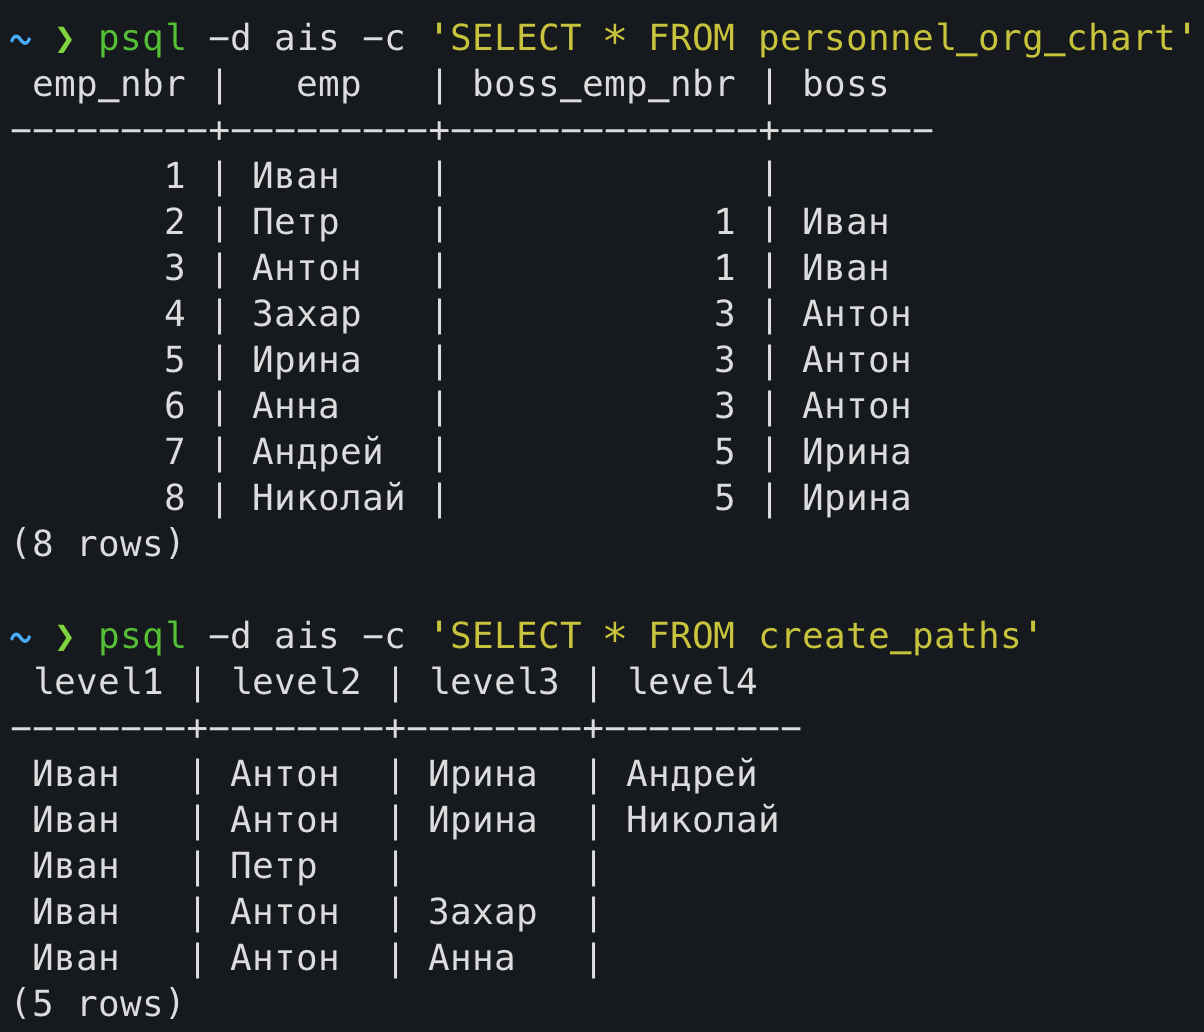
\includegraphics[scale=0.7]{12_3.png}
\end{center}
\clearpage
\section*{Номер 13}
\begin{center}
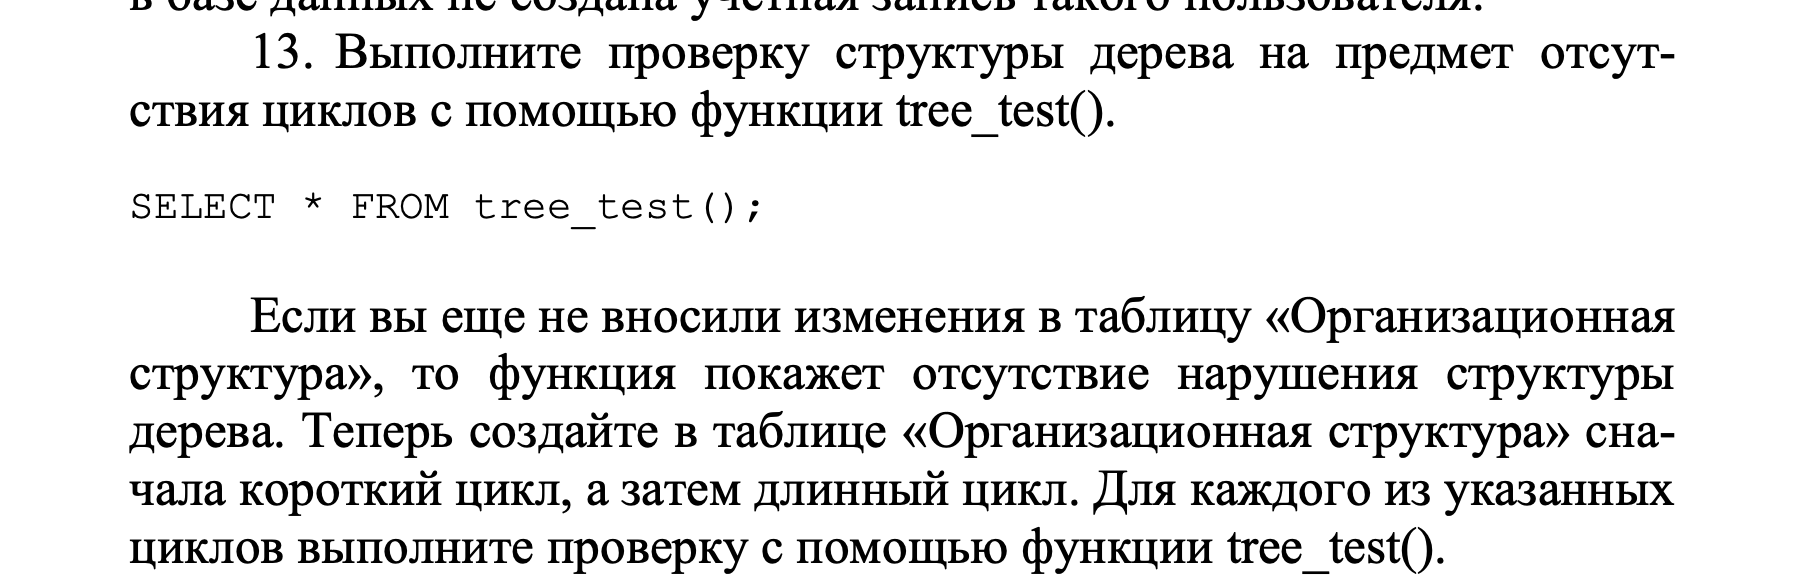
\includegraphics[scale=0.5]{13_1.png}
\end{center}
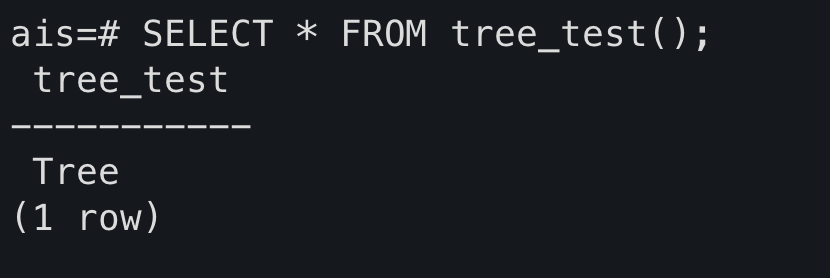
\includegraphics[scale=0.8]{13_2.png}
\\\\
Первый раз:
\begin{flushleft}
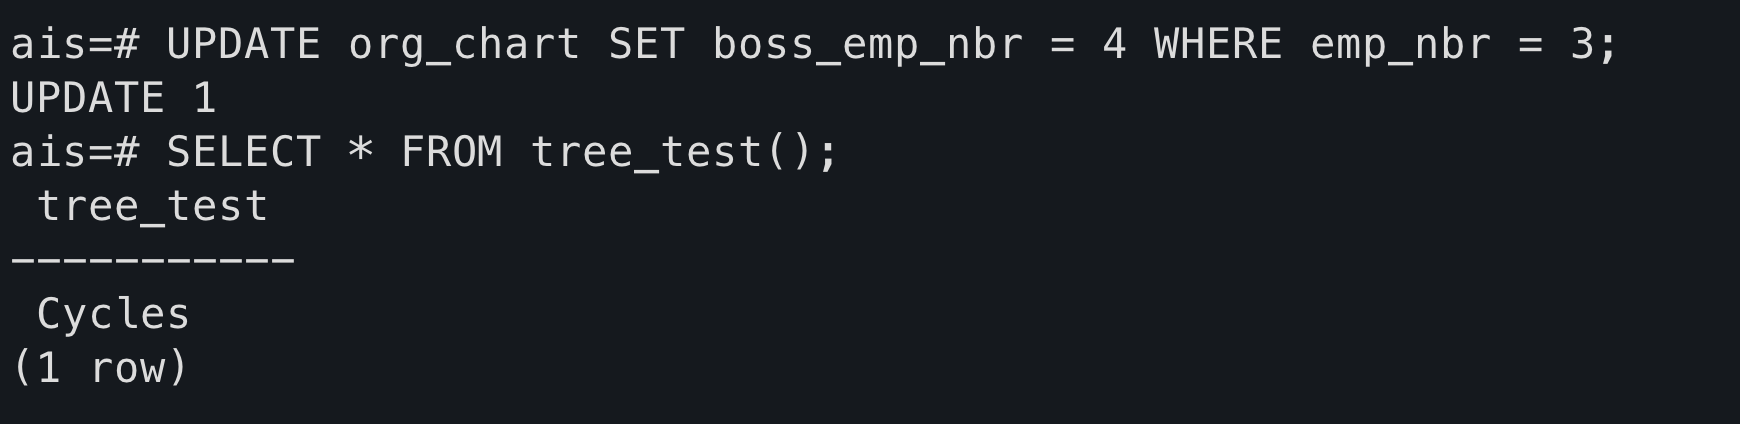
\includegraphics[scale=0.6]{13_3.png}
\end{flushleft}
Второй раз:
\begin{flushleft}
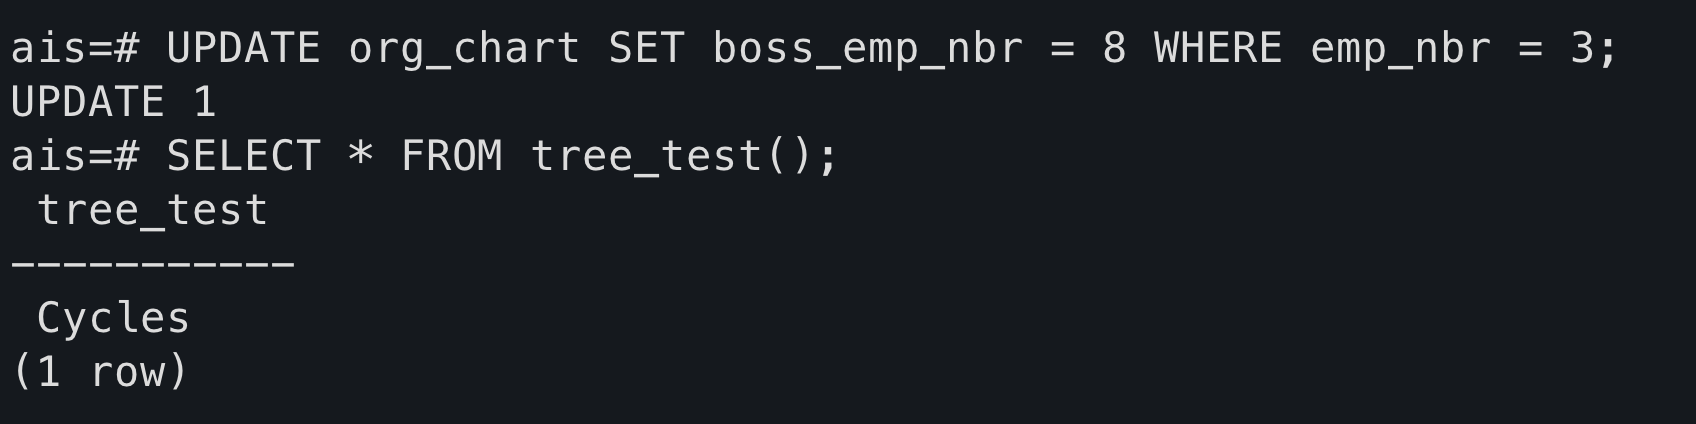
\includegraphics[scale=0.6]{13_4.png}
\end{flushleft}
\clearpage
\section*{Номер 14}
\begin{flushleft}

\includegraphics[scale=0.6]{14_1.png}
\end{flushleft}
\begin{flushleft}
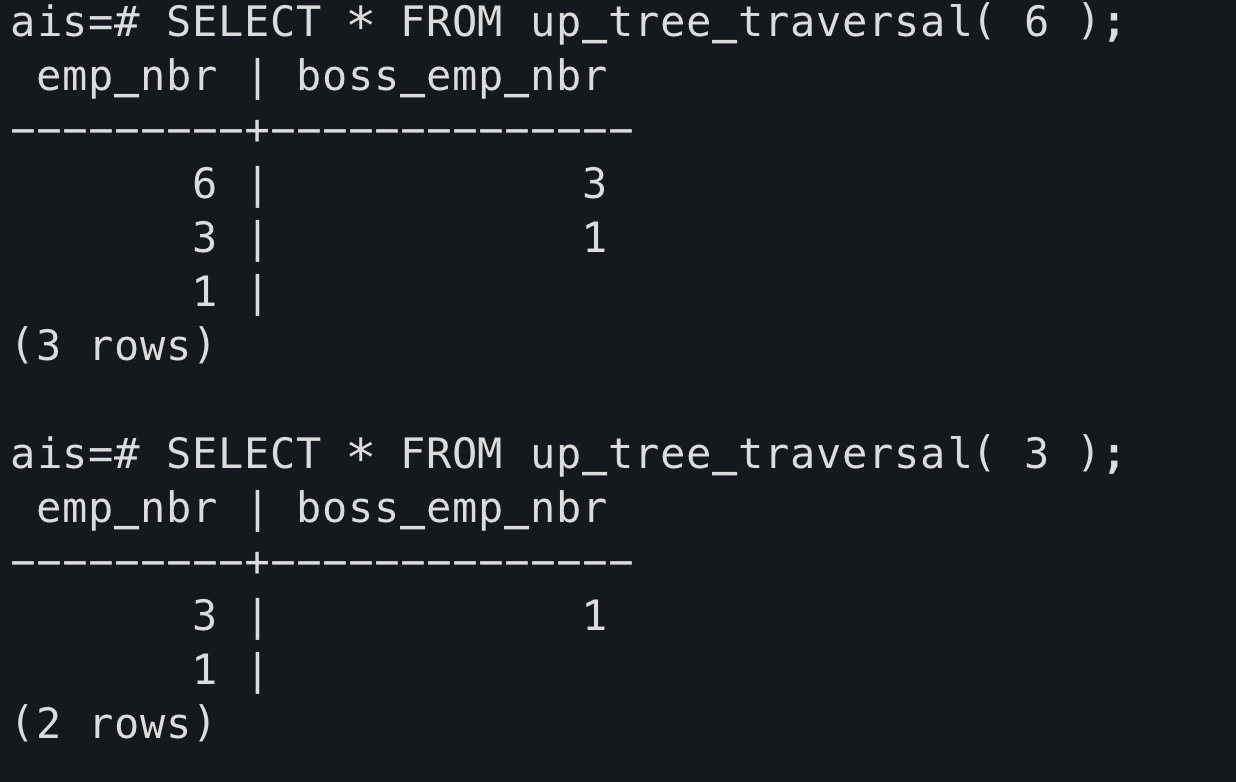
\includegraphics[scale=0.5]{14_2.png}
\end{flushleft}
\begin{flushleft}
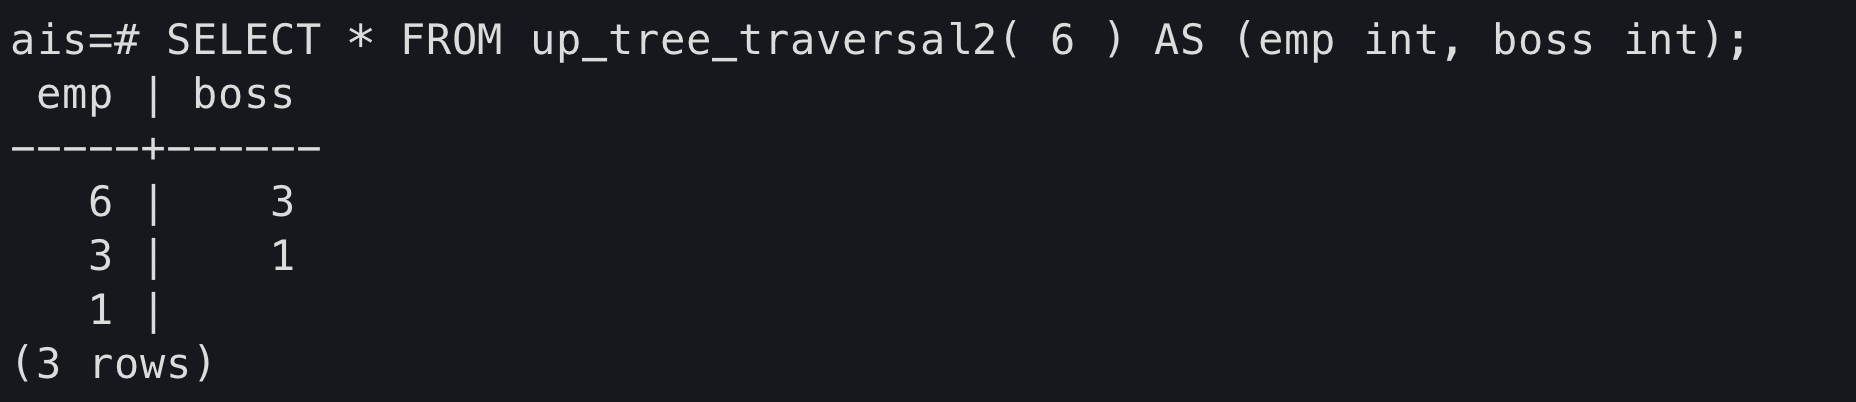
\includegraphics[scale=0.5]{14_3.png}
\end{flushleft}
\begin{flushleft}
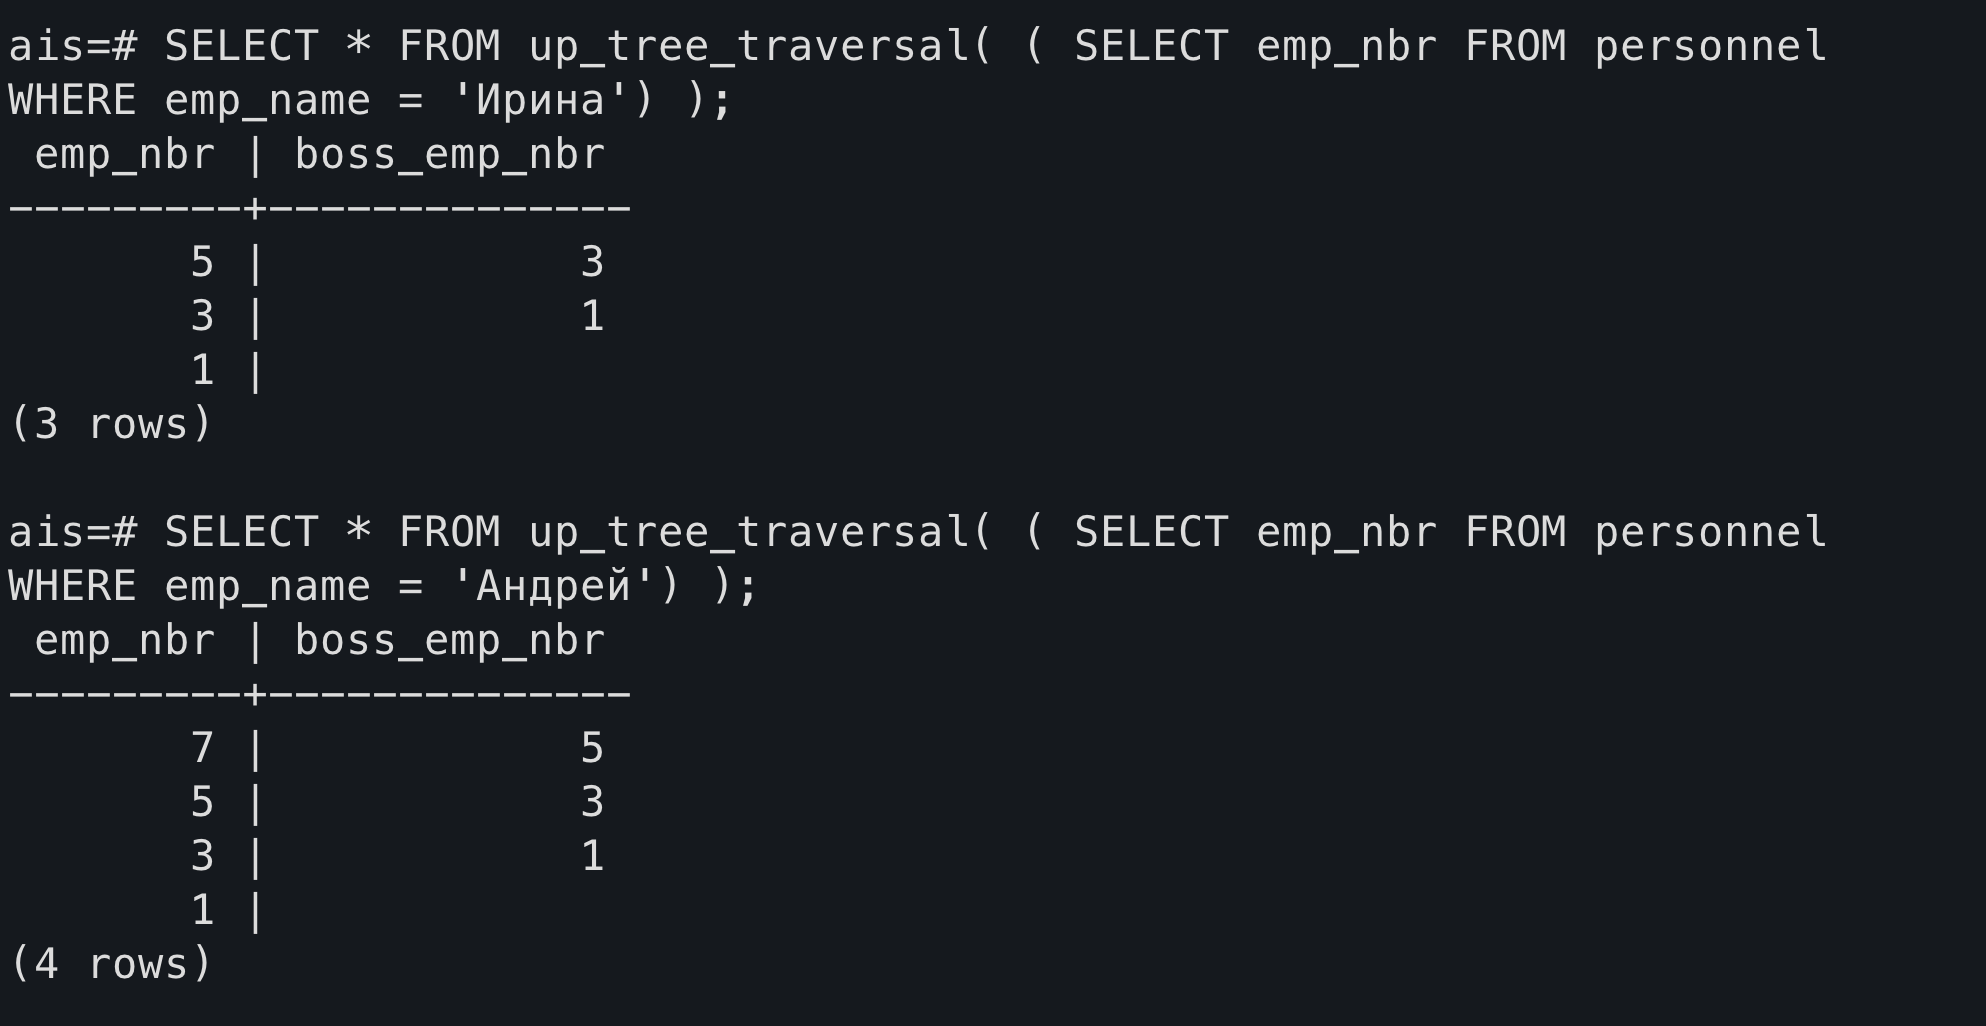
\includegraphics[scale=0.5]{14_4.png}
\end{flushleft}
\clearpage
\section*{Номер 15}
\begin{flushleft}
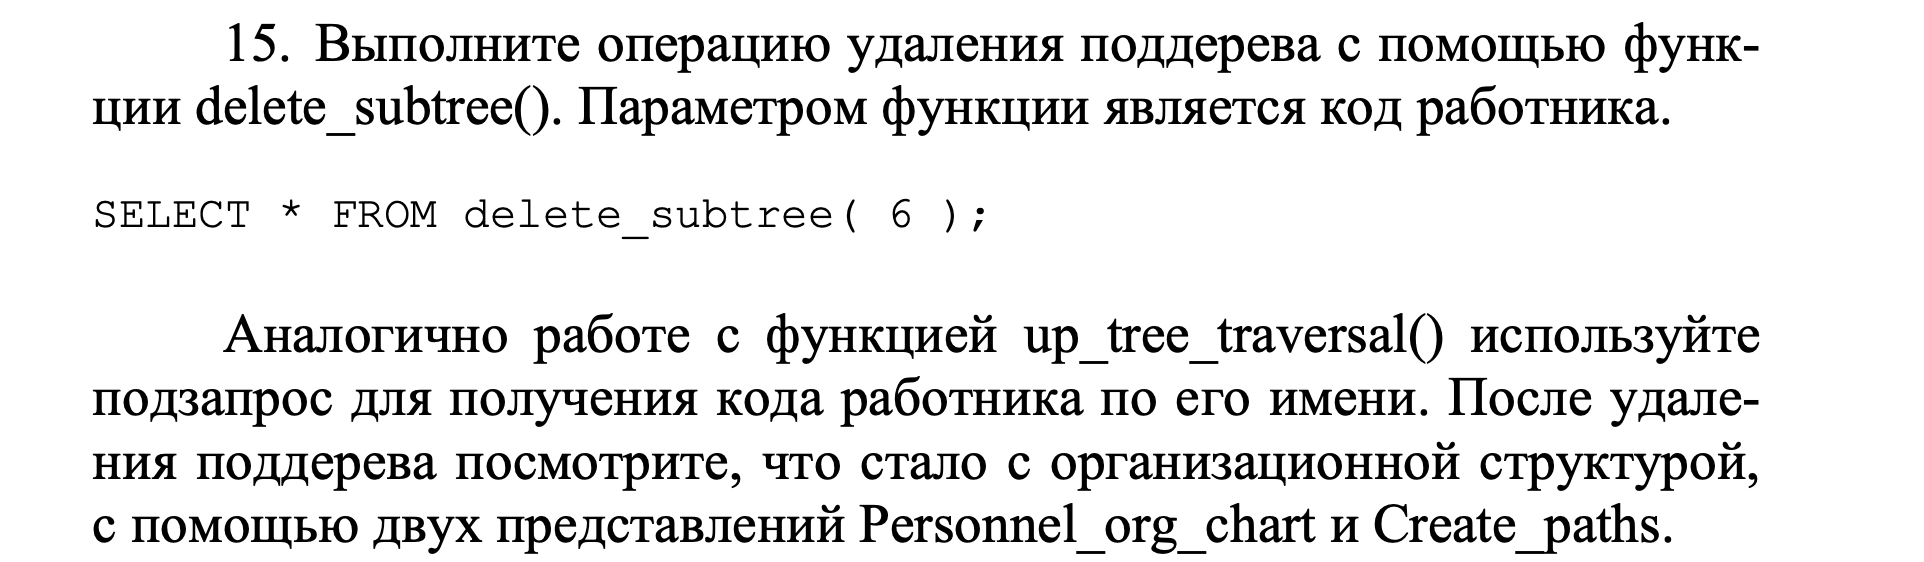
\includegraphics[scale=0.5]{15_1.png}
\end{flushleft}
Изначальное состояние:
\begin{flushleft}
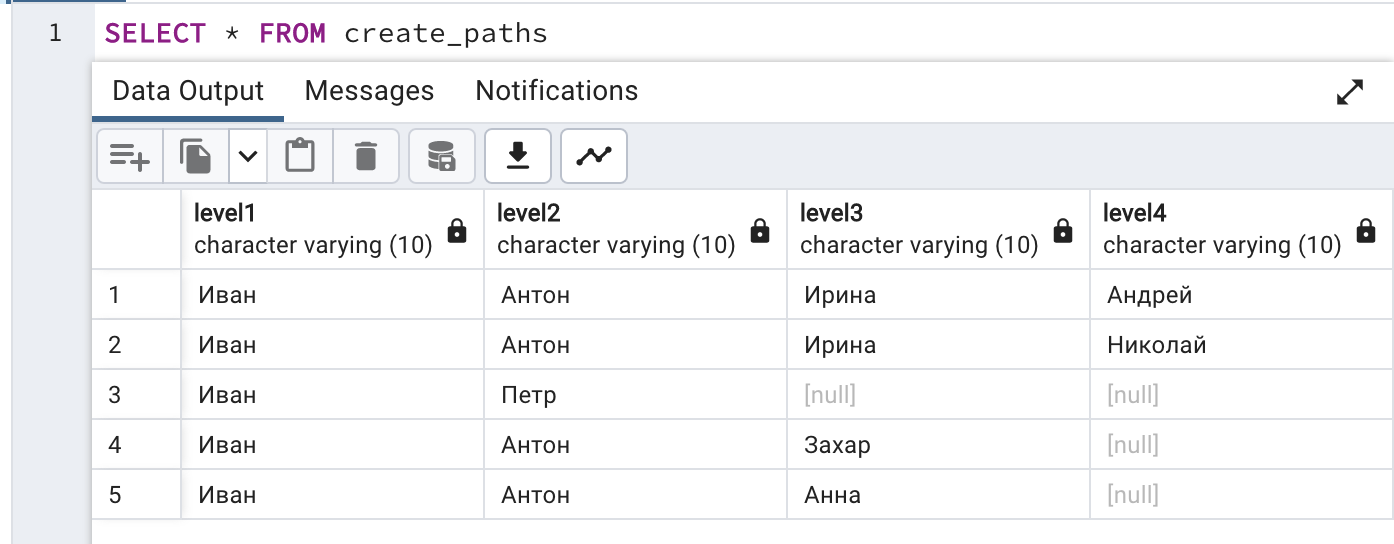
\includegraphics[scale=0.5]{15_2.png}
\end{flushleft}
\begin{flushleft}
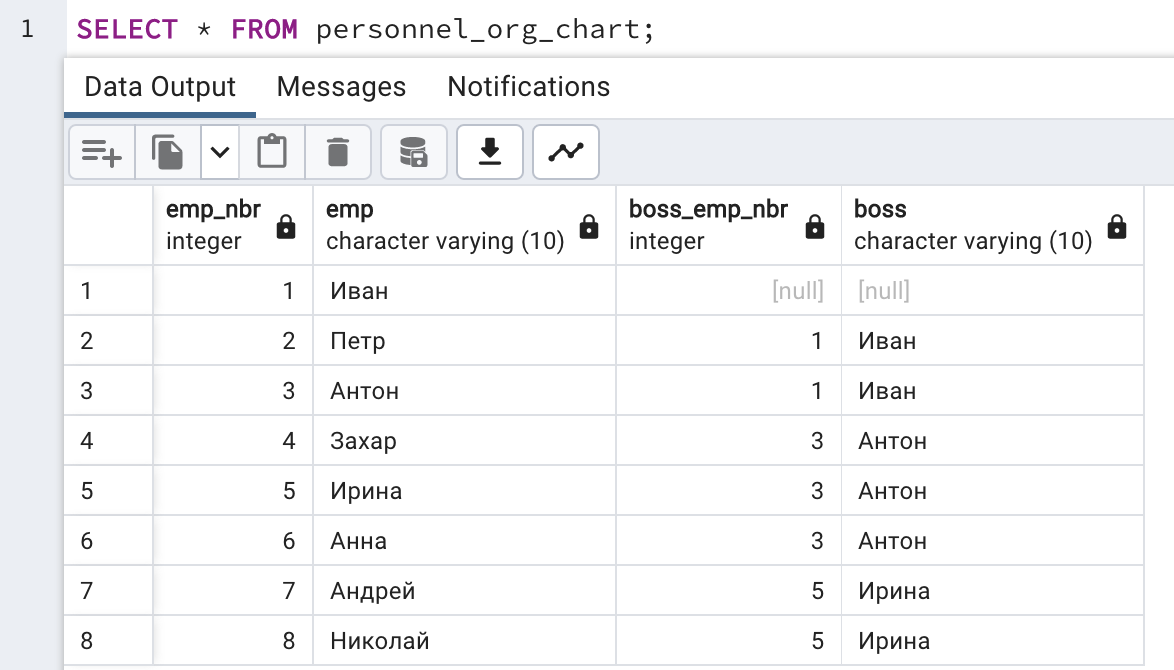
\includegraphics[scale=0.6]{15_3.png}
\end{flushleft}
Проводим запрос:
\begin{flushleft}
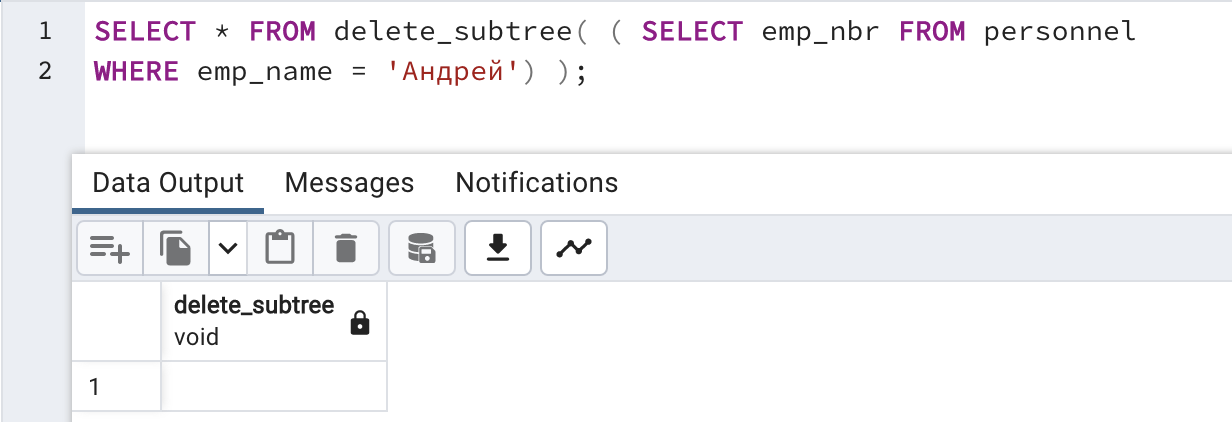
\includegraphics[scale=0.5]{15_4.png}
\end{flushleft}
Новое состояние:
\begin{flushleft}
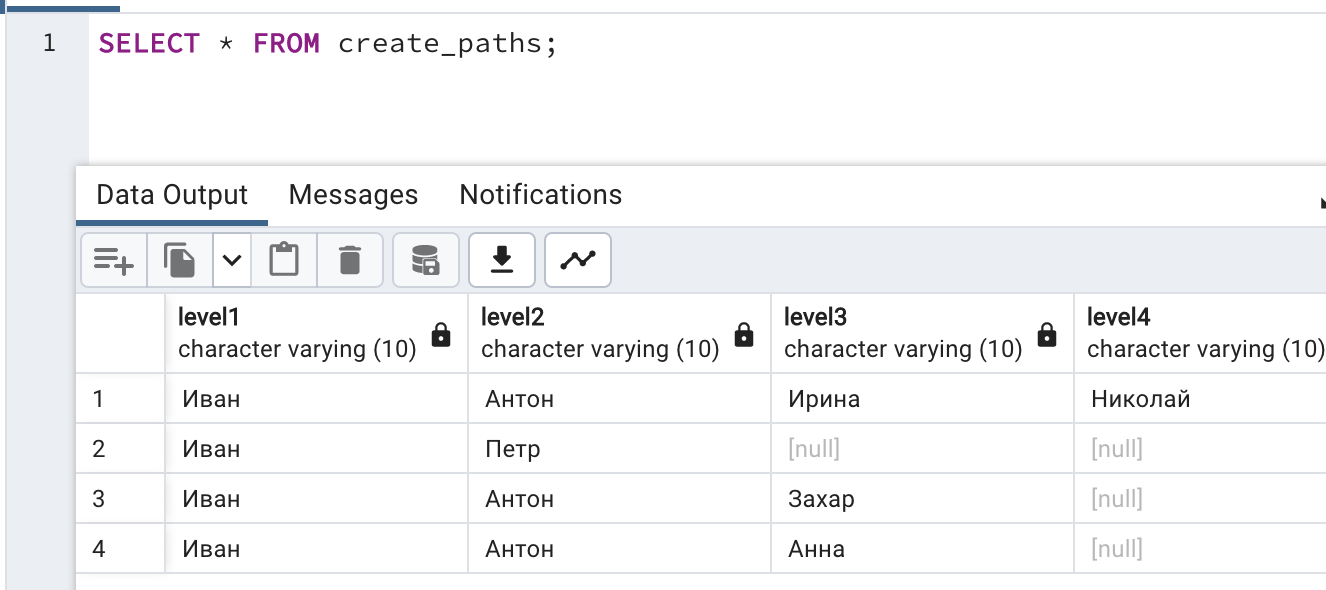
\includegraphics[scale=0.5]{15_5.png}
\end{flushleft}
\begin{flushleft}
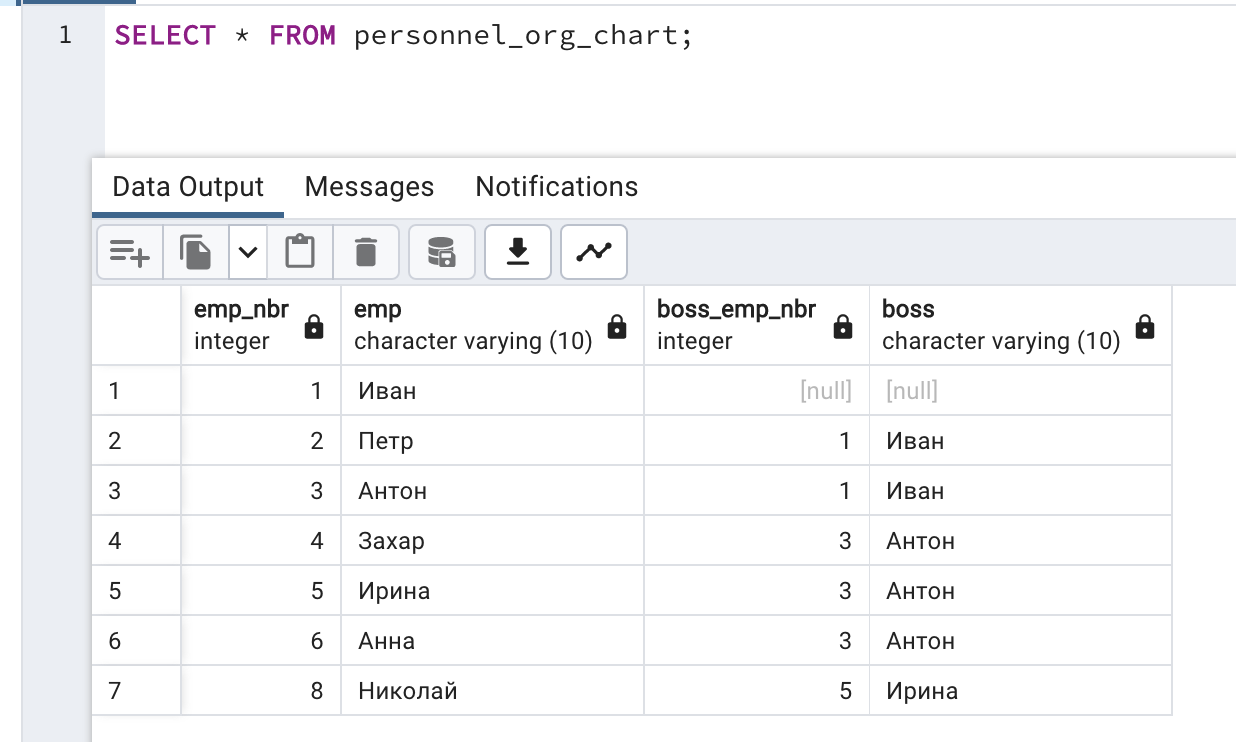
\includegraphics[scale=0.5]{15_6.png}
\end{flushleft}
\clearpage
\section*{Номер 16}
\begin{flushleft}
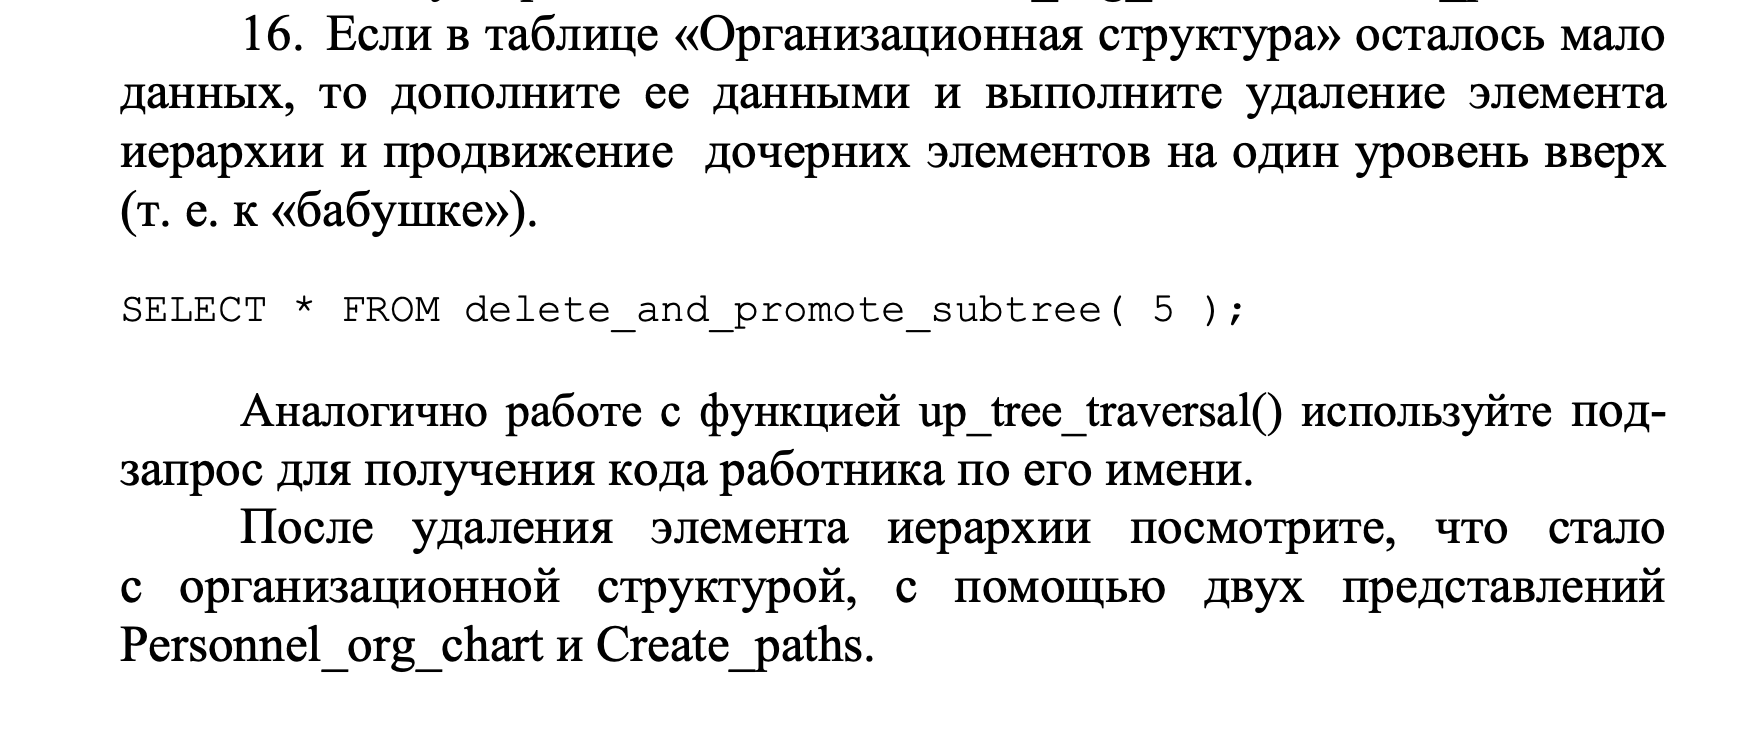
\includegraphics[scale=0.5]{16_1.png}
\end{flushleft}
Провожу запрос:
\begin{flushleft}
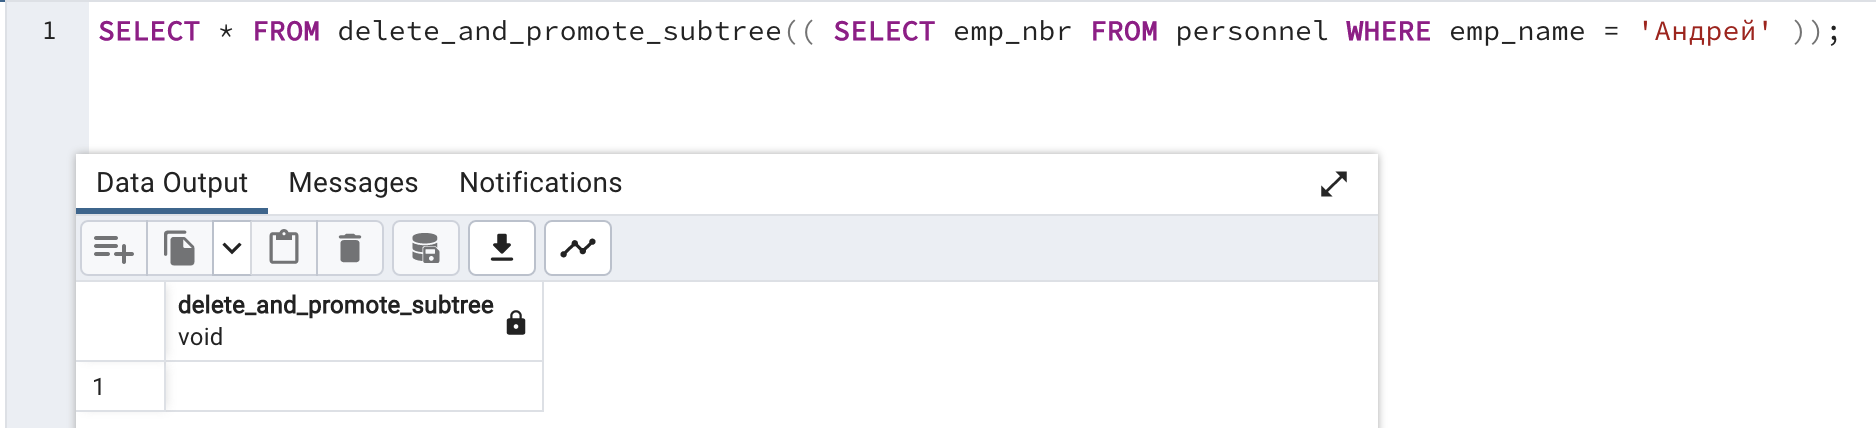
\includegraphics[scale=0.5]{16_2.png}
\end{flushleft}
Смотрю состояния:
\begin{flushleft}
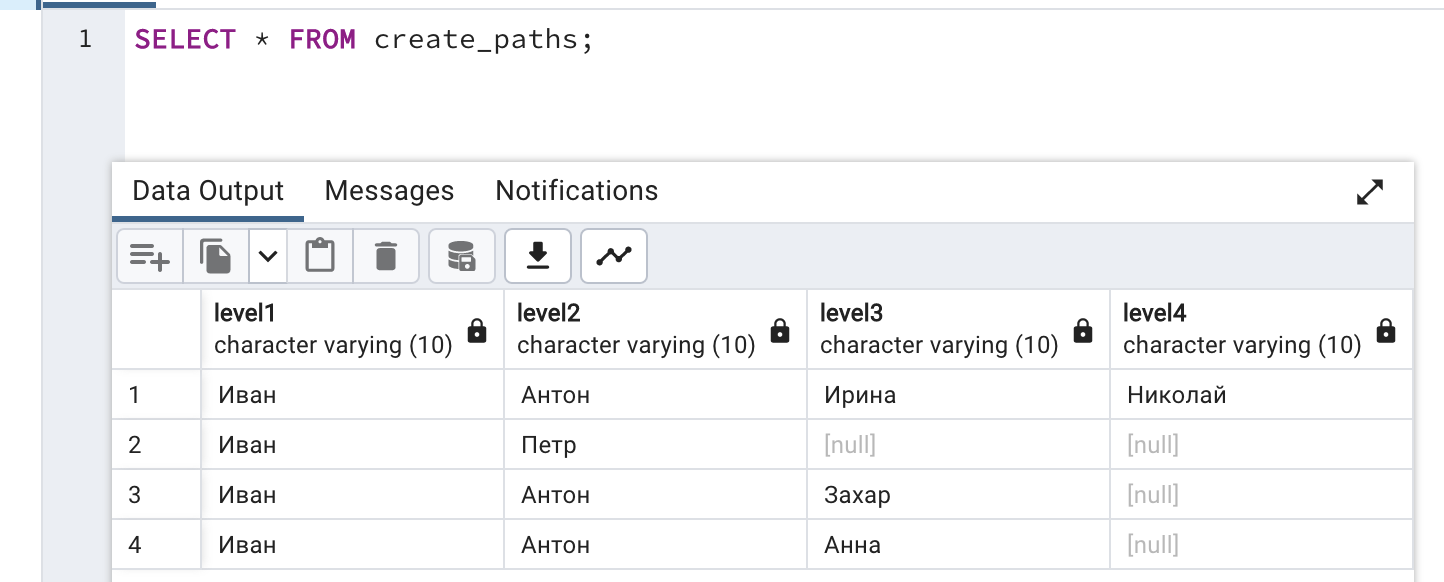
\includegraphics[scale=0.5]{16_3.png}
\end{flushleft}
\begin{flushleft}
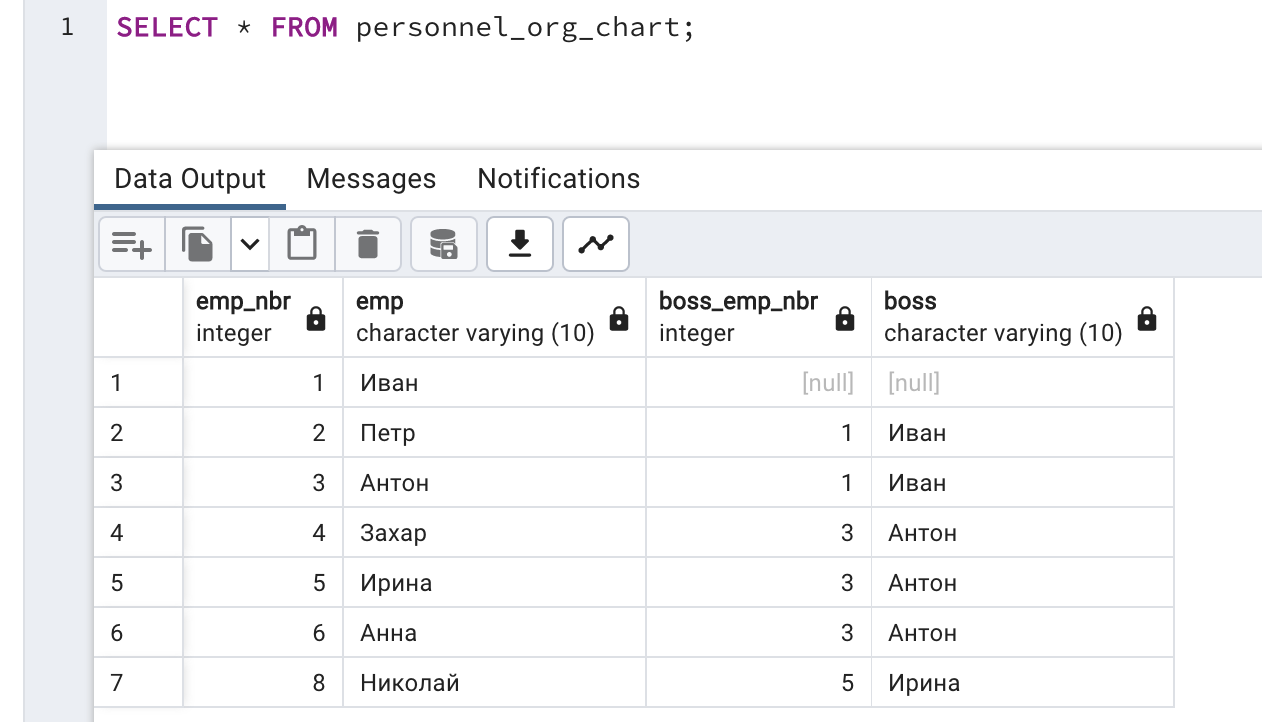
\includegraphics[scale=0.5]{16_4.png}
\end{flushleft}
\clearpage
\section*{Номер 17}
\begin{flushleft}

\includegraphics[scale=0.5]{17_1.png}
\end{flushleft}
Создаю представление
\begin{flushleft}
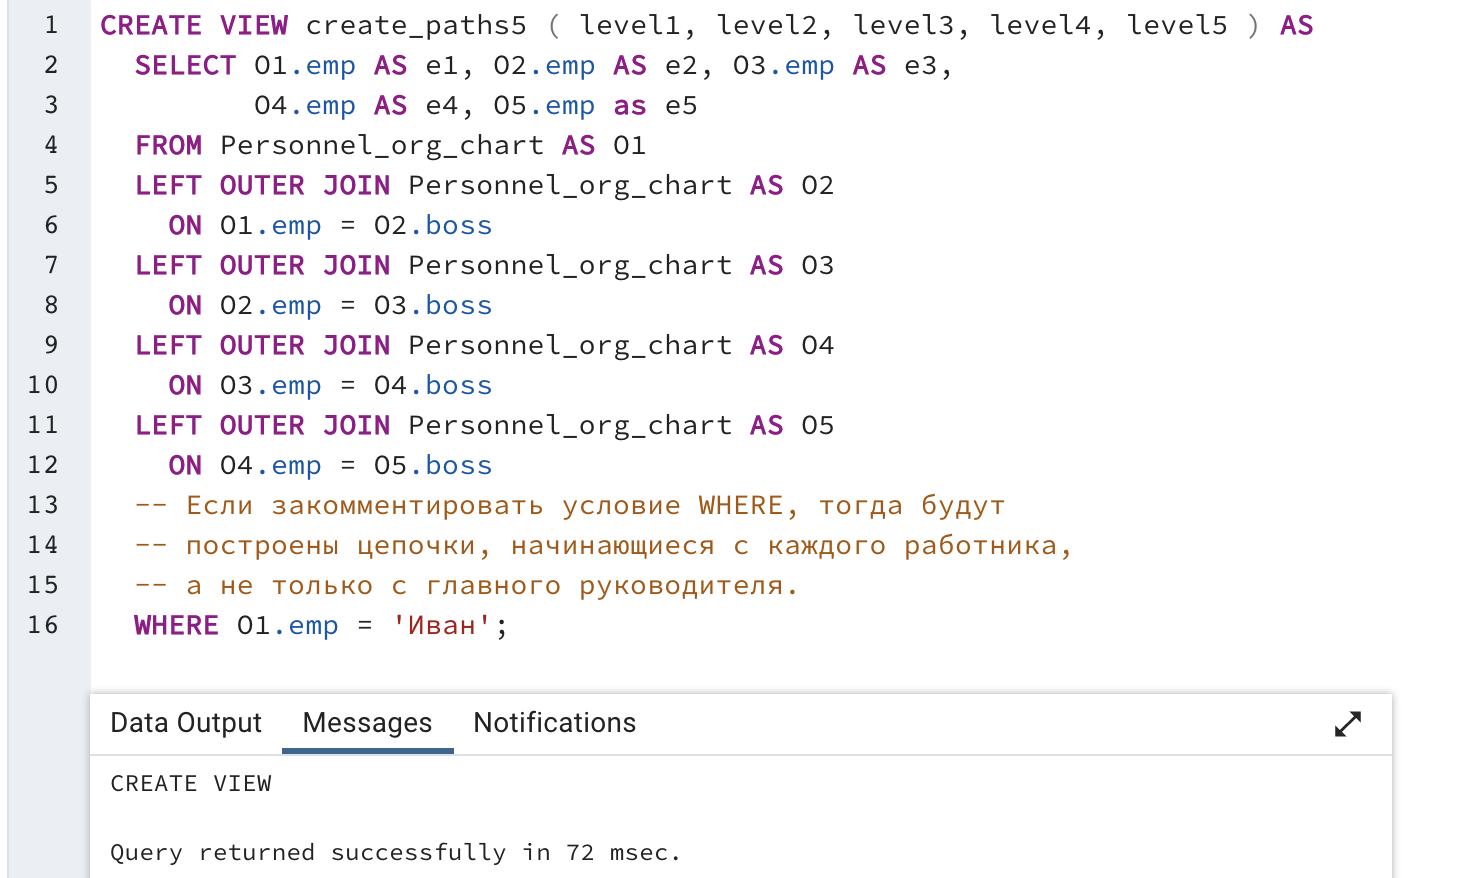
\includegraphics[scale=0.5]{17_2.png}
\end{flushleft}
Смотрю вывод:
\begin{flushleft}
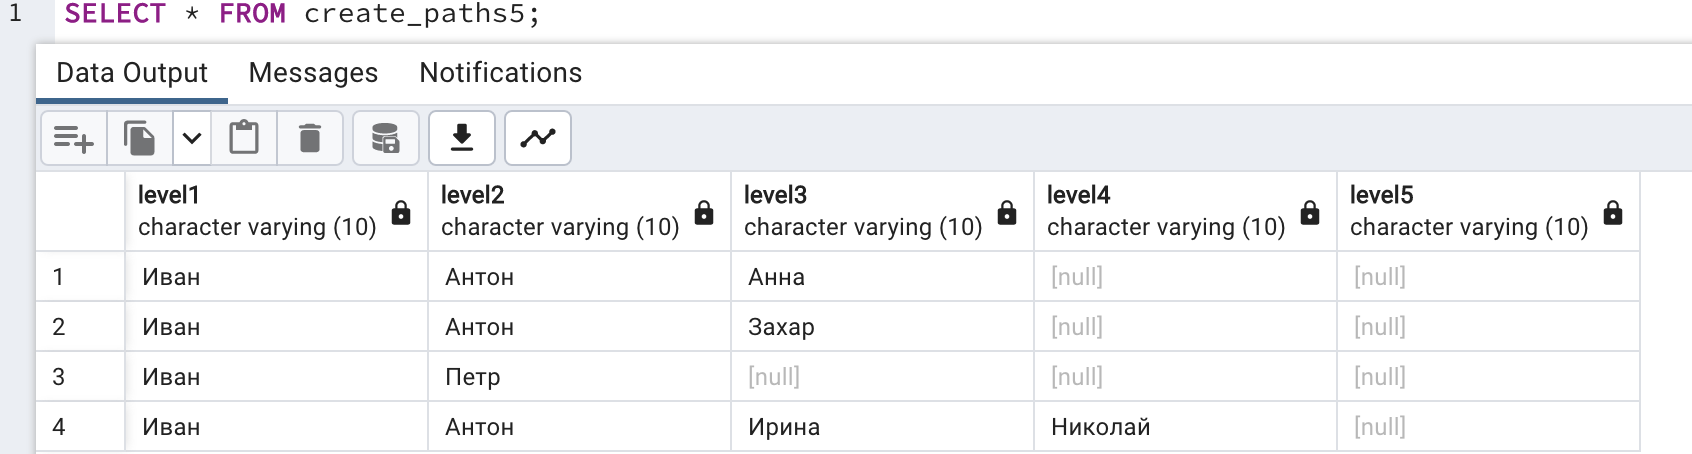
\includegraphics[scale=0.5]{17_3.png}
\end{flushleft}
\clearpage
\section*{Номер 18}
\begin{flushleft}

\includegraphics[scale=0.5]{18_1.png}
\end{flushleft}
В качестве примера решил создать функцию с курсором, которая  показывает, родился ли человек в четный день месяца. Исходно создал новую колонку в таблице и заполнил ее False. Сама функция:
\begin{flushleft}
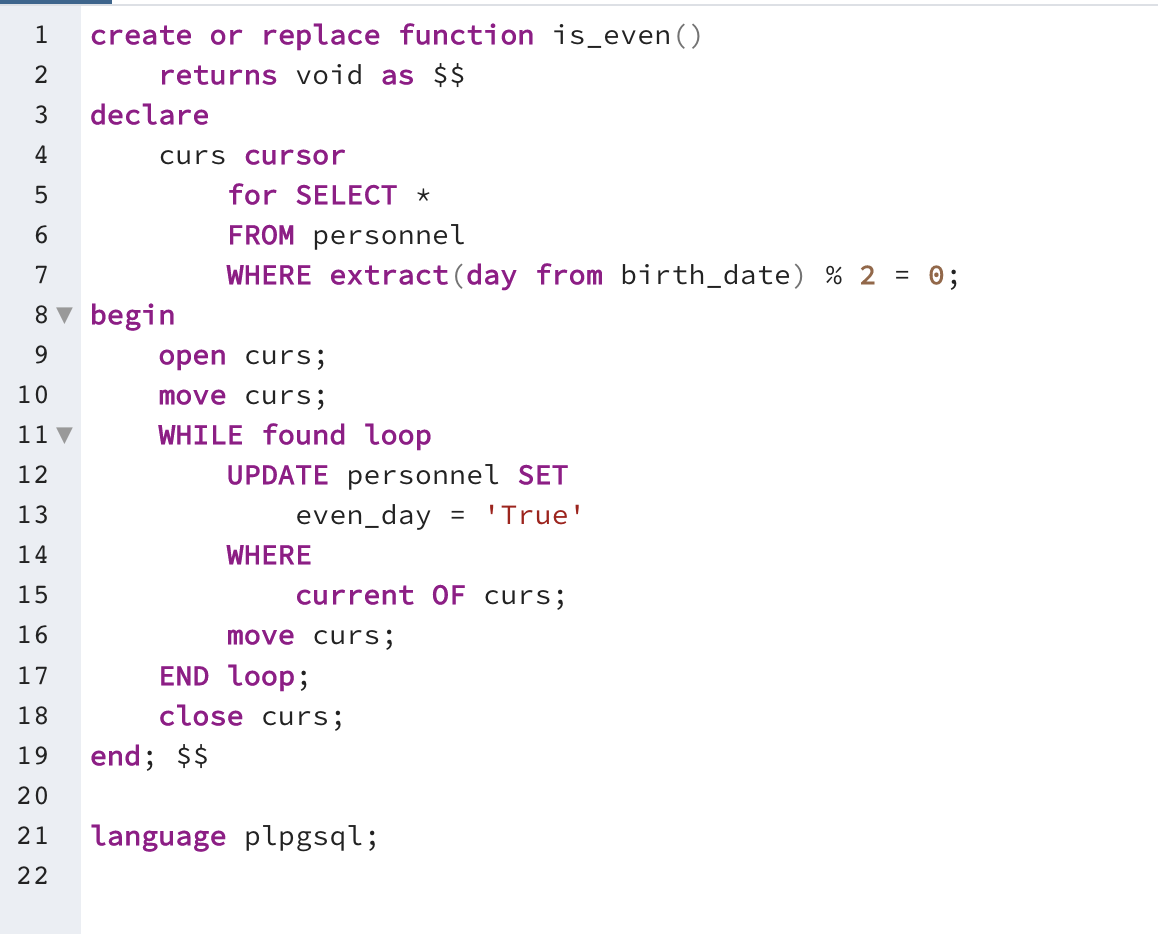
\includegraphics[scale=0.6]{18_2.png}
\end{flushleft}
Исходное состояние до вызова функции:
\begin{flushleft}
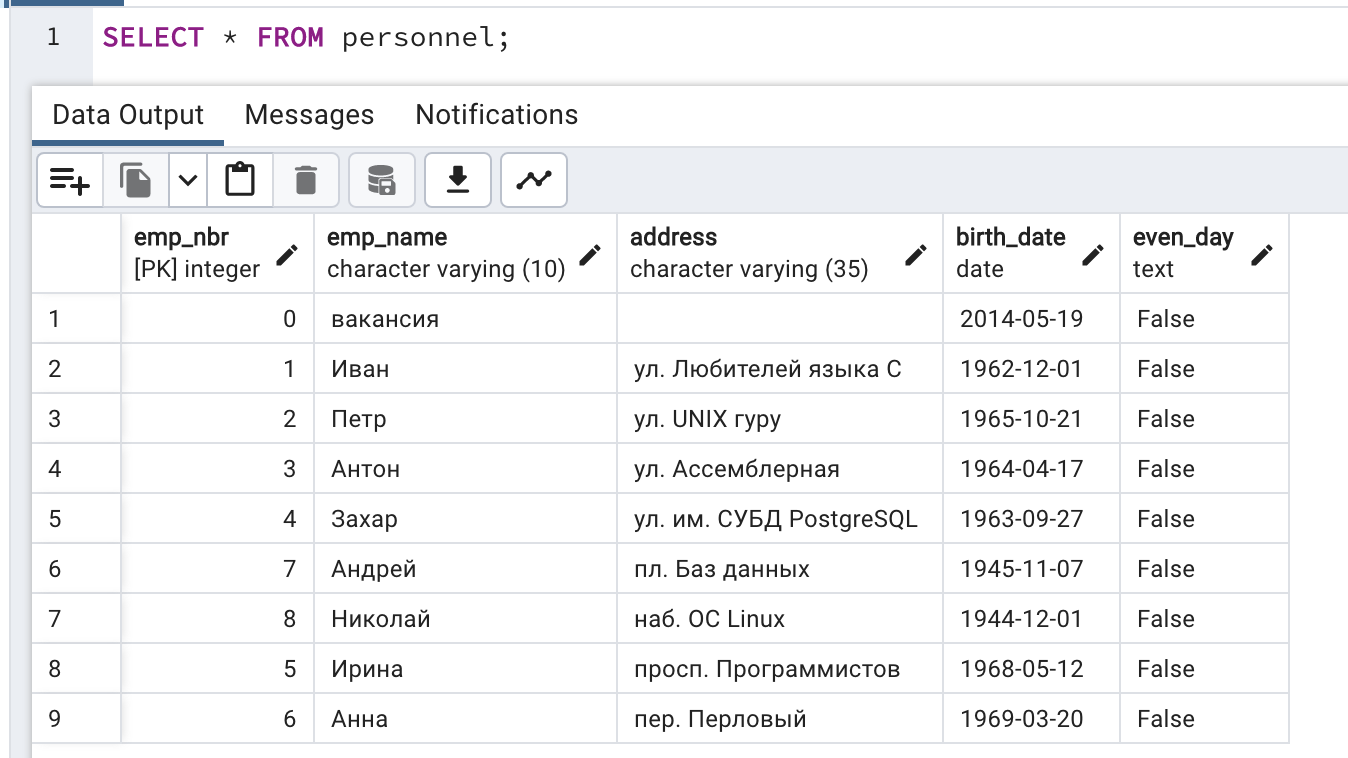
\includegraphics[scale=0.6]{18_3.png}
\end{flushleft}
Вызываю функцию:
\begin{flushleft}
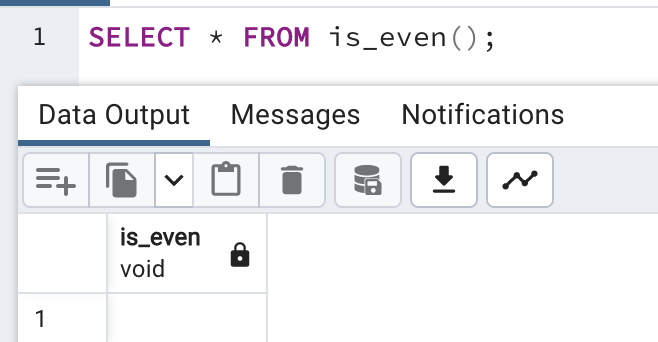
\includegraphics[scale=0.6]{18_4.png}
\end{flushleft}
Смотрю на результат:
\begin{flushleft}
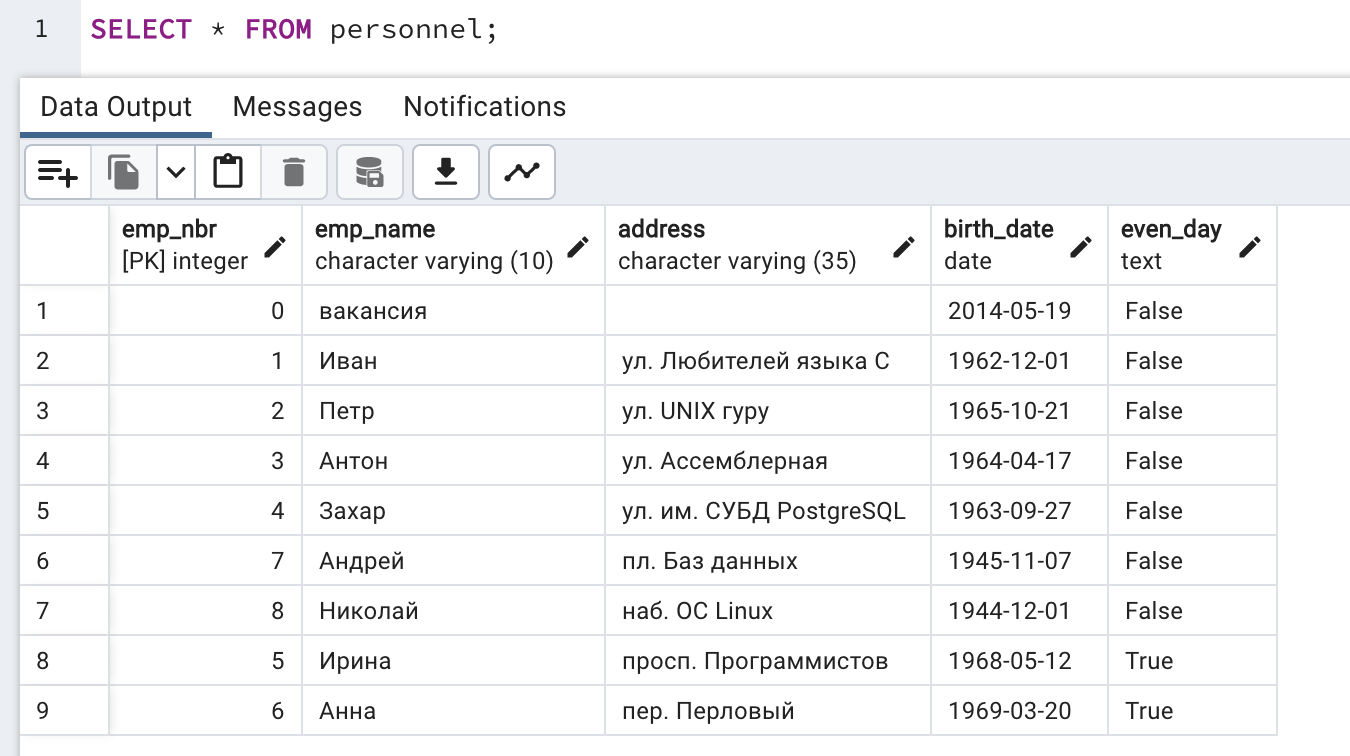
\includegraphics[scale=0.6]{18_5.png}
\end{flushleft}
у людей с четными днями рождения теперь графа равна True
\end{document}
